\subsection{Emergency Path Planning}\label{sub_section:tgt_path_planning}

\subsubsection{Cost Function}\label{sub_sub_section:tgt_cost_function}
The key objective is to reduce the downtime and cost of operation of the drone. This means both the cost of damage to the drone through crashing and the difficulty of retrieval need consideration. Considering the centre of each hexagon in the cost map as a node and modelling the probability of surviving half of a node-to-node traversal between adjacent nodes as the constant $p$, the cost function of any path of length $D$ is shown in Equation \ref{eq:cost function}. The specific $c_{\text{crashing}}$ and $c_{\text{landing}}$ can be defined by the ground operators for each classification. The ones used in testing are shown in Table \ref{tab:cost_values}.
\begin{equation}\label{eq:cost function}
    E(x) 
    = \sum_{n=1}^{D-1} c_{\text{crashing}}\bigl(x_n\bigr)\, (1-p) \,p^n 
    \;+\; c_{\text{landing}}\bigl(x_D\bigr)\, p^D
\end{equation}
\begin{table}[h]
    \centering
    \begin{tabular}{|c|c|c|c|c|}
    \hline
         \textbf{} & \textbf{Safe} & \textbf{Semi-Dangerous} & \textbf{Dangerous} & \textbf{Obstacle} \\
         \hline
         $c_{\text{landing}}$ & 0 & 1 & 10 & 100 \\
         $c_{\text{crashing}}$ & 10 & 10 & 100 & 1000\\
         \hline
    \end{tabular}
    \caption{Testing Costs}
    \label{tab:cost_values}
\end{table}

\subsubsection{Weather induced failure}\label{sub_sub_section:tgt_weather_failure}
\paragraph{Cause}
When a gust of wind exceeds the control capabilities of the drone it will cause an extreme disturbance and likely failure resulting in a crash. This is especially important to consider when their is an actuator fault as the maximum rejected gust becomes lower in magnitude and therefore more likely to occur.
\paragraph{Wind Speed Modelling}
To model the wind in the operational environment, a wind speed monitor is deployed at base stations. Wind speeds are measured at 1 Hz in m/s. For a given time, $\tau$ we can a gust vector $\mathbf{x_{\tau}} =  \{x_1, x_2, \dots, x_N\}$ where $x_i$ is the max wind speed in that time. The wind speed is then modelled using the Weibull distribution \cite{weibull1951} with PDF given by Equation \ref{eq:weibull_pdf}.
\begin{equation}\label{eq:weibull_pdf}
    f_X(x; k, \lambda) = \frac{k}{\lambda} \left(\frac{x}{\lambda}\right)^{k-1} \exp\left(-\left(\frac{x}{\lambda}\right)^k\right),
\end{equation}
where:
\begin{itemize}
    \item \( k > 0 \): Shape parameter (controls skewness),
    \item \( \lambda > 0 \): Scale parameter (characteristic wind speed).
\end{itemize}
The probability that a gust exceeds \( v \) in any given second is derived from the Weibull survival function shown in Equation \ref{eq:weibull_survive}.
\begin{equation}\label{eq:weibull_survive}
    P(X > v) = 1 - F_X(v) = \exp\left(-\left(\frac{v}{\lambda}\right)^k\right).
\end{equation}
The model $k, \lambda$ parameters are estimated by calculating the Maximum Likelihood Estimation of Equation \ref{eq:weibull_likilihood} using numerical methods such as Newton-Raphson \cite{rinne2008}.
\begin{equation}\label{eq:weibull_likilihood}
     \mathcal{L}(k, \lambda) = \prod_{i=1}^N f_X(x_i; k, \lambda)
\end{equation}
\paragraph{Calculating $p$}
The maximum wind speed rejection, $v$, is a known parameter for all deployed controllers discussed in Section \ref{sub_sub_section:tgt_actuator_fault}. From this, we can calculate $p$ as discussed in Section \ref{sub_sub_section:tgt_cost_function} in Equation \ref{eq:p_calc}; $\tau$ is set as the expected travel time for the characteristic distance of $p$.
\begin{equation}\label{eq:p_calc}
    p = 1-P(X>v)
\end{equation}
\paragraph{Deployment}
For each deployed controller, there is a defined maximum wind speed rejection $v$ and travel speed $s$. For a cost map, the half-nodal distance for $p$, $d$, is also predefined. Therefore, we can calculate $\tau$ based on given we know the controller deployed on the drone using $\tau = d/s$. This can then be used to calculate a $p$ using data from the last $50\tau$ data points to balance recency with noise rejection. This can be calculated continuously on the base station to give a live approximation. Using the LoRa communication system already deployed, the system shown in Figure \ref{fig:wind_process} is used, where the device sends out the controller it is using to the base-station, $p$ is calculated on the base station and sent back to the device. This system, to the best of the author's knowledge, is not currently deployed, and so real-world performance testing is required.
\begin{figure}[htbp]
  \centering
  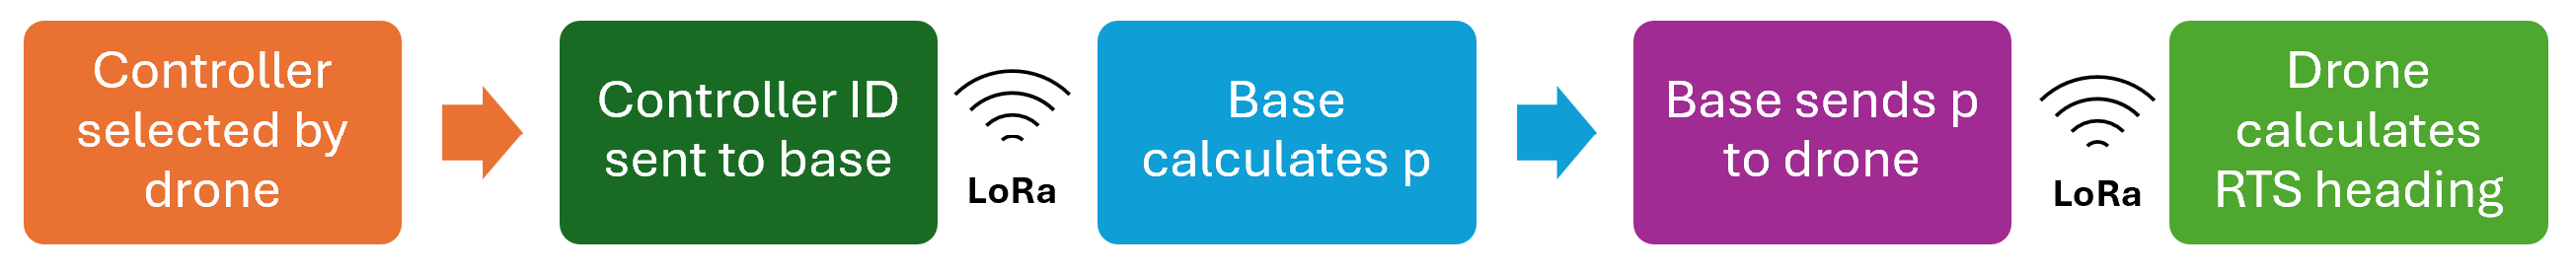
\includegraphics[width=\textwidth]{figs/Thomas/Return To Safety/wind_process.png}
  \caption{Wind speed RTS process}
  \label{fig:wind_process}
\end{figure}

\subsubsection{Path Planning}\label{sub_sub_section:tgt_search}
%\begin{algorithm}
\caption{Exhaustive Search}
\label{alg:search}
\begin{algorithmic}[1]
    \For{each Node $n$}
        \State $\textit{min\_cost} \gets \infty$
        \State $n.path\_cost$ = \Call{search}{$n$, $p$, $1$, $0$, $depth$, $\textit{min\_cost}$}
    \EndFor
    
    \Function{search}{$n$, $p$, $p\_alive$, $cost$, $depth$, \textbf{ref} $\textit{min\_cost}$}
        \State $\textit{current\_cost} \gets cost + p\_alive \cdot n.\textit{landing\_cost}$
        \If{$\textit{current\_cost} < \textit{min\_cost}$}
            \State $\textit{min\_cost} \gets \textit{current\_cost}$
        \EndIf
        \If{$depth = 0$ $\mathbf{or}$ $n.\textit{landing\_cost} = 0$ $\mathbf{or}$ $cost > \textit{min\_cost}$}
            \State \Return
        \EndIf
        \For{each $\textit{neighbour}$ in $n.\textit{neighbours}$}
            \State $p\_alive\_next \gets p\_alive \cdot p$
            \State $cost\_next \gets cost + p\_alive \cdot (1 - p) \cdot n.\textit{crashing\_cost}$
            \State \Call{search}{$\textit{neighbour}$, $p$, $p\_alive\_next$, $cost\_next$, $depth - 1$, $\textit{min\_cost}$}
        \EndFor
    \EndFunction
\end{algorithmic}
\end{algorithm}
\begin{algorithm}
    \caption{Smooth}
    \label{alg:flow}
\begin{algorithmic}[1]
    \While{not $Converged$}
        \State $Converged \gets TRUE$
        \For{each Node $n$}
            \For{each \textit{neighbour} in $n.\textit{neighbours}$}
                \State $\textit{movement\_cost} \gets n.\textit{crashing\_cost} \cdot \frac{1 - p}{2} +  \textit{neighbour}.\textit{crashing\_cost} \cdot \frac{p(1 - p)}{2}$
                \State $\textit{total\_cost} \gets \textit{movement\_cost} + p \cdot \textit{neighbour.path\_cost}$
                \If{$\textit{total\_cost} < n.\textit{path\_cost}$}
                    \State $n.\textit{path\_cost} \gets \textit{total\_cost}$
                    \State $Converged \gets FALSE$
                \EndIf
            \EndFor
        \EndFor
    \EndWhile
\end{algorithmic}
\end{algorithm}
\paragraph{Pre-Compute}
Carrying out memory and time complex operations on real-time hardware should always be avoided as operations require specific timings for optimal use. If all the values are pre-computed and uploaded to the device, the time and memory complexity becomes $O(1)$, which supports precise, timed operations. Within the path planning workflow, as much as possible should be pre-computed and simply accessed; however, if any algorithms are deployed, they should be $O(1)$.
\paragraph{$p$ ranges}
While the value of $p$ can take any value between 0 and 1, there can be only 7 outputs for the next best move (going to each of the 6 neighbours or landing). Therefore, instead of creating a specific map for a specific value of $p$ on the flight controller, you can pre-compute all the ranges of $p$ that would cause each of these outcomes. Then the device selects the option corresponding to its current $p$ value.
\paragraph{Map}
\begin{figure}[htbp]\label{fig:rts_complexity}
  \centering
  \begin{subfigure}[b]{0.48\textwidth}
    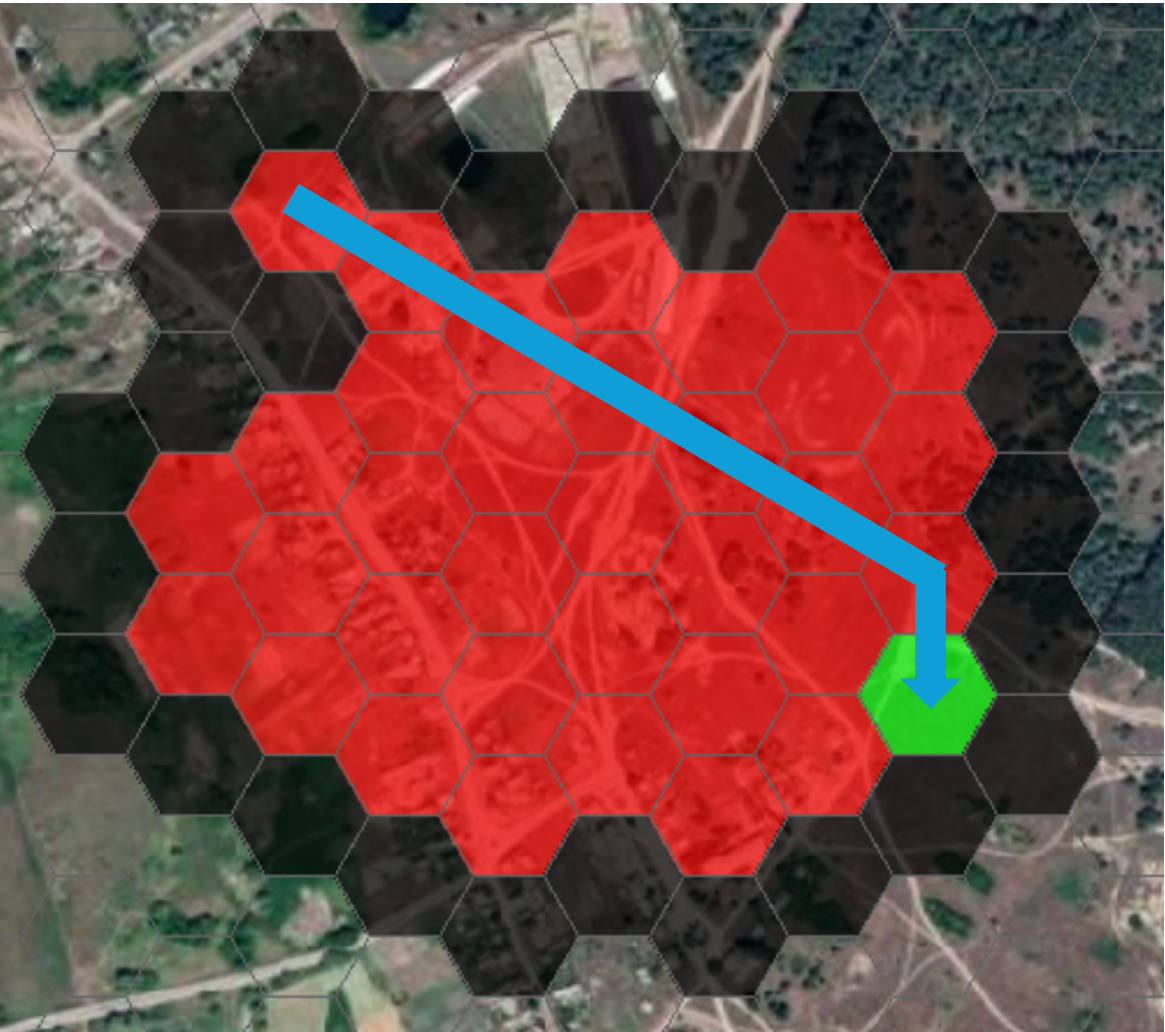
\includegraphics[width=\textwidth]{figs/Thomas/Return To Safety/typical_case_complexity.png}
    \caption{Typical Case RTS Complexity}
    \label{fig:typical_case}
  \end{subfigure}
  \hfill
  \begin{subfigure}[b]{0.48\textwidth}
    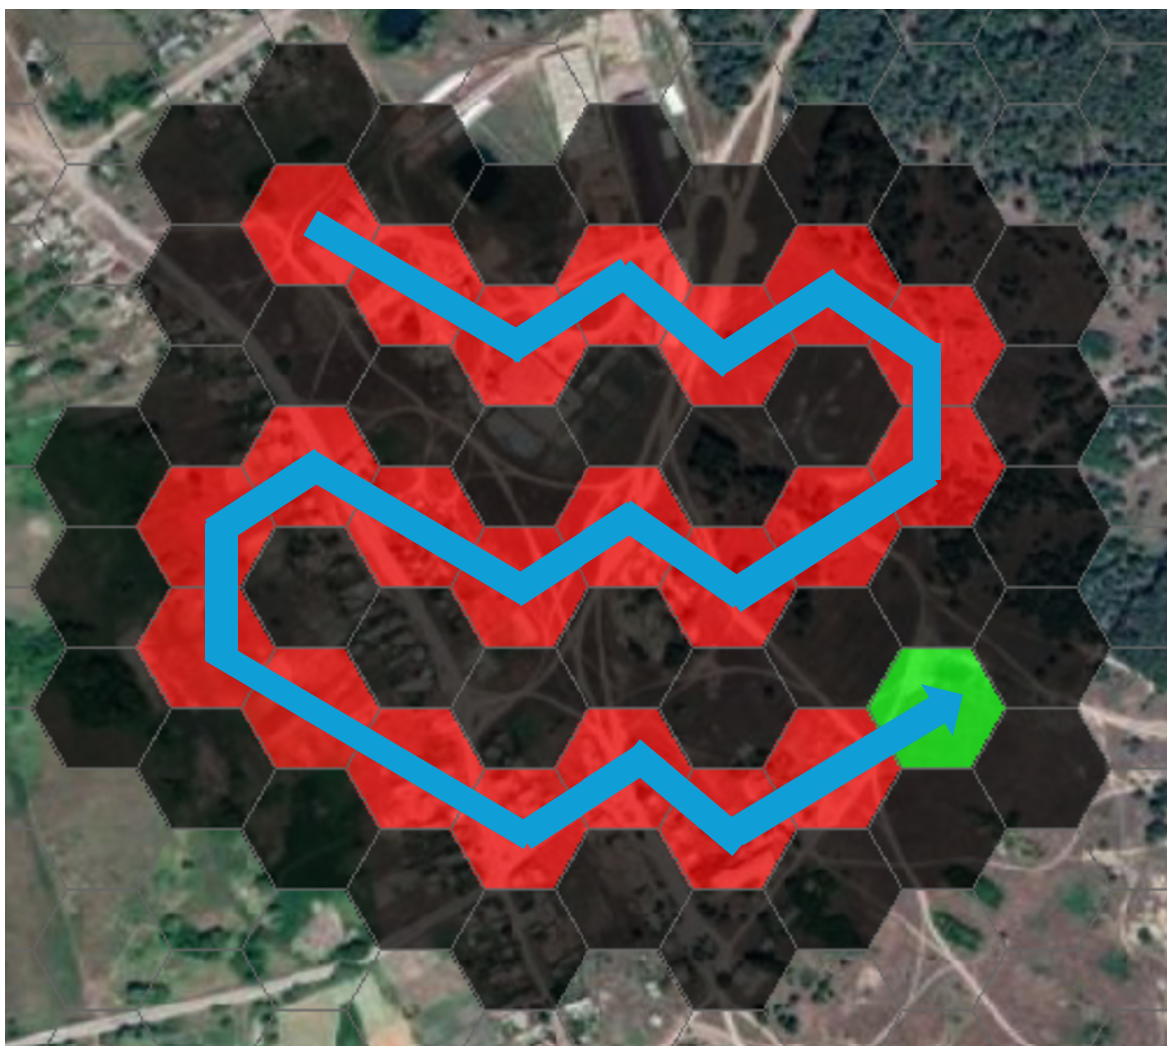
\includegraphics[width=\textwidth]{figs/Thomas/Return To Safety/worst_case_complexity.png}
    \caption{Worst Case RTS Path Complexity}
    \label{fig:worst_case}
\end{subfigure}
\caption{RTS Complexity}
\end{figure}
To minimise on-board compute, a map is uploaded where it simply tells the device where to go next, given the value of $p$ and its current position. To calculate this, the optimal next-node must be calculated for $p\in[0\to1]$ with a suitable step size (0.01 was used in testing).  To calculate the optimal next node for all nodes at a specified value of $p$, I developed Algorithm \ref{alg:flow}. This is based on a Bellman-Ford \cite{bellman1958}\cite{ford1956} approach and therefore restricts the system to non-negative cycles; however, given that this is a damage mitigation task, having non-negative costs is to be expected.
\paragraph{Complexity}
Bellman-Ford algorithms have a worst-case time complexity of $O(|E|\times |V|)$ where $|V|$ represents the longest path length. We know $|E| \leq |V| \times 7$ and is therefore $O(|V)$ as we are using hexagons that can have an edge to 6 neighbours and a self-edge indicating landing. Therefore, the actual worst-case complexity is $O(|V|^2)$\cite{cormen2009}.  Furthermore, as seen in Figure \ref{fig:rts_complexity} in the best-case, the longest path length is $O(\sqrt{|V|})$, reducing the best-case complexity to $O(|V|^{1.5})$. 

\paragraph{Dijkstra}
The complexity of Dijkstra's algorithm \cite{dijkstra1959} with priority queue for similarly sparse maps is $O(|E| + |V|log|V|)$ however it is not appropriate as Algorithm \ref{alg:flow} has recursive dependencies making edge weights non-static violating the greedy condition \cite{cormen2009}. 
\subsubsection{Real-time application}\label{sub_sub_section:tgt_real_time}
\paragraph{Deployment}
For a deployed algorithm, consistent timings and a minimal memory footprint are essential. Algorithm \ref{alg:threshold} is used to select the next action based on the value of $p$ and the node $p$ ranges.
\begin{algorithm}[htbp]
  \caption{Threshold-Based Action Selection}
  \label{alg:threshold}
  \begin{algorithmic}[1]
    \Require Sorted threshold array \(\mathcal{P} = [p_1, p_2, \dots, p_6]\), associated actions \(\mathcal{A} = [a_1, a_2, \dots, a_6]\), input probability \(p\), default landing action \(a_{\textit{land}}\)
    \Ensure Selected action \(a\), GNSS coordinates \((\textit{lat}, \textit{lon})\)
    
    \State \(a \gets a_{\textit{land}}\) \Comment{Default to landing}
    \For{\(i = 1\) to \(n\)}
      \If{\(p < p_i\)}
        \State \(a \gets a_i\)
        \State \textbf{break}
      \EndIf
    \EndFor
    
    \State \((\textit{row}, \textit{col}) \gets \textit{GridCoordinates}(a)\)
    \State \((\textit{lat}, \textit{lon}) \gets \Call{ConvertToGNSS}{\textit{row}, \textit{col}}\)
    
    \State \Return \((a, \textit{lat}, \textit{lon})\)
  \end{algorithmic}
\end{algorithm}
\paragraph{Memory Management}
The memory on the \gls{MCU}s consists of Flash and \gls{SRAM}. Flash is static memory that has to be pre-loaded onto the board before each run, whereas \gls{SRAM} is volatile but has faster access times. Therefore, waypoints, maps, and gains are loaded into \gls{RAM} from the preset values in Flash before a flight. In addition, the flight controller's \gls{MCU} has \gls{ITCM} configured \gls{RAM} and \gls{DTCM} configured \gls{RAM}. \gls{DTCM} and \gls{ITCM} allow for precise timings when accessing data and instructions respectively\footnote{\url{https://developer.arm.com/documentation/107565/0101/Memory-system/Tightly-Coupled-Memory--TCM-}} and should therefore be used for looped processes, including control loops and heading calculations. Whereas, for less timing critical actions or varying time operations such as actuator tests, the regular \gls{SRAM} can be used. For the \gls{GNSS} module \gls{MCU}, there is just Flash and \gls{SRAM}; however, as it is a less complex operational loop, this is sufficient. 
\begin{table}[h]
\centering
\begin{tabular}{ccccc} 
\toprule
\textbf{Device}&\textbf{Flash}&\textbf{SRAM}&\textbf{DTCM}&\textbf{ITCM}\\
 & (megabytes)& (kilobytes)& (kilobytes)& (kilobytes)\\
\midrule
STM32H743VGT6\tablefootnote{\url{https://www.st.com/en/microcontrollers-microprocessors/stm32h743vg.html}}&1&1000&128&64\\
MSPM0G3506SRHBR\tablefootnote{\url{https://www.ti.com/product/MSPM0G3506/part-details/MSPM0G3506SRHBR}}&0.128&64&-&-\\
\bottomrule
\end{tabular}
\caption{MCU Memory}
\label{tab:MCU_memory}
\end{table}

\paragraph{Memory Reduced Nodes}
Using a C implementation as shown in Listing \ref{lst:node}, it requires 56 bytes per node; therefore, for a 256-node map it requires 14.336 kilobytes of \gls{RAM}. This puts significant resolution limitations on the map. Therefore, the map should be stored in custom data structures that contain only as many bits as required. By using an indexed node array instead of pointers, 12-bit indexes can be used, supporting 4096 nodes, and 8 bits for probability values is sufficient. Lastly, the index of the node can be used to derive its location, removing the relative values. This structure is shown in Listing \ref{lst:reducednode} and with the above values and using a guaranteed optimal number of thresholds and actions of 6, results in 16.5 bytes per node. However, the major drawback is that when moving away from standard C data types, bespoke bit operations are required, increasing the development difficulty. 
\paragraph{Stop-Go Method}
The nature of the problem can be exploited using the strategy of the map having one option for the next move that above a probability threshold it goes to, and below that threshold it lands. This means that only one action and one threshold in the Listing \ref{lst:reducednode} reduced node structure is needed, resulting in a memory intensity of 4 bytes per node.
\newpage
\begin{lstlisting}[caption={Implementated Node Structure},label={lst:node}]
struct Node {
    float rel_long, rel_lat;  // relative longitude and latitude to reference point
    float p_values[6];        // Probability thresholds
    Node* actions[6];         // Points to the next node
};
\end{lstlisting}
\begin{lstlisting}[caption={Node Structure},label={lst:reducednode}]
struct Node {
    idx;           // Current Index Position
    p_values[];    // Probability thresholds
    actions[];     // Indexes of the next node
};
\end{lstlisting}

\paragraph{Testing}
Using 10 random satellite images from the Kharkiv region, 256 node cost maps were generated, including visible obstacles and assumed regions of interest. Each trail consisted of starting at each node in the region of interest and finding the actual cost, using the values given in Table \ref{tab:cost_values}, experienced following maps generated by each nodal structure for a specified value of $p$. 20 trials were run per interval between $p$ values 0.01 and 0.99 with intervals of 0.01, and the aggregate average performances between Stop-Go, Reduced, and Implemented nodes were all within 0.01\% showing equivalent performance of each nodal structure over the dataset. However, the Stop-Go method can no longer guarantee optimal results, leaving them vulnerable to unforeseen situations and varying cost functions. Therefore, the reduced node given in Listing \ref{lst:reducednode} should be implemented unless there are significant memory requirements. Further field validation is required as the dataset used may be different from a real-world application.



\begin{comment}
\paragraph{Exhaustive Search}
The simplest algorithm is the recursive function shown in Algorithm \ref{alg: search}. There are steps taken to increase the efficiency, including pruning lines that already exceed the minimum cost as the cost is monotonic increasing, and automatically terminating lines when they can land safely. However, the worst-case time complexity remains $O(|V|6^{depth})$ as each node has 6 neighbours that get called recursively. To get guaranteed correct results, it would require searching all paths as long as $|V|$, as costs cannot fall below 0, so it is never advantageous to revisit a node. Therefore, the worst-case complexity for guaranteed optimal paths is $O(|V|6^{|V|})$. This is not usable for practical applications, therefore, it requires a compromise on the depth of search, no longer getting optimal path results.
\end{comment}